%\section{Markov Inequality, 2015-08-16}
%\label{2015-08-16:entry}

\DiaryEntry{Markov and Chebyshev Inequality}{2015-08-16}{Stochastic}

holds for non-negative random variable $X$ and $a > 0$. Consider an indicator function $I(\cdot)$ which is one when the condition is true and zero otherwise. Now distinguish between the two cases $X \geq a$ and $X < a$. If $X \geq a$, then $I(X \geq a) = 1$; if $X < a$, then $I(X \geq a) = 0$. We can collect this in a single expression, namely
%
\begin{equation*}
a I(X \geq a) \leq X
\end{equation*}
%
Taking expectation on both sides yields
%
\begin{equation*}
a \mathrm{E}(I(X \geq a)) \leq \mathrm{E}(X)
\end{equation*}
%
and we observe that $a \mathrm{E}(I(X \geq a)) = P(X \geq a)$ and therefore we have
%
\begin{equation*}
a P(X \geq a) \leq \mathrm{E}(X) \rightarrow P(X \geq a) \leq \frac{\mathrm{E}(X)}{a}
\end{equation*}
%
which is the famous Markov inequality.


\subsection*{Example}

Example for the exponential distribution $f(x) = \lambda e^{- \lambda x}$ as follows:
%
\begin{equation*}
P(X \geq a) =  \int_a^\infty \lambda e^{- \lambda x} = e^{- \lambda a}
\end{equation*}
%
The expectation is $E(X) = 1/\lambda$ and therefore we have
%
\begin{equation*}
P(X \geq a) \leq \frac{1}{\lambda a}
\end{equation*}
%
In the plot below the green curve shows the true value of $P(X \geq a)$; the blue curve is the Markov approximation.

\begin{figure}[h]
\centering
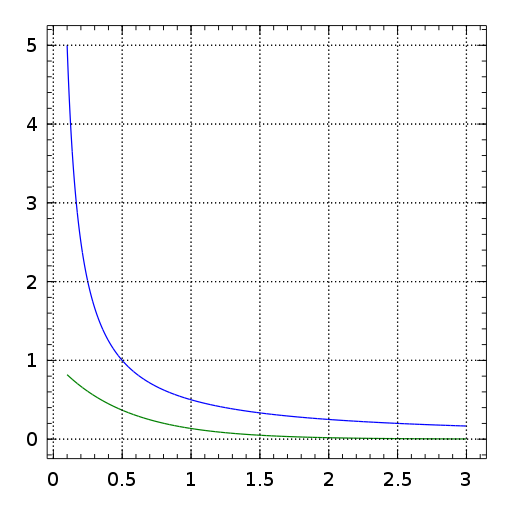
\includegraphics[scale=0.35]{images/exponential.png}
\caption{Exponential Distribution: Tail probabilities.}
\end{figure}

\subsection*{Chebyshev Inequality}

Whereas the Markov inequality holds only for positive RV's and requires only a known mean, the Chebyshev inequality holds for any RV with known (and existing) mean and variance.

We consider the absolute value of a RV $|X|$. Using the Markov inequality, we have
%
\begin{equation*}
  P(|Y| \geq a) \leq \frac{\mathrm{E}\{|Y|\}}{a}
\end{equation*}
%
We now consider a RV $Y = (X - \mu)^2$ and $a = (k \sigma)^2$ (where $\mu$ is the expectation of $X$ and $\sigma^2$ its variance) and we obtain
%
\begin{equation*}
  P(|X-\mu|^2 \geq (k \sigma)^2) \leq \frac{\mathrm{E}\{(X-\mu)^2\}}{(k \sigma)^2} = \frac{\sigma^2}{k^2 \sigma^2} = 1 / k^2
\end{equation*}
%
%
We therefore arrive at the Chebyshev inequality
%
\begin{equation*}
    P(|X-\mu|^2 \geq (k \sigma)^2) \leq 1 / k^2
\end{equation*}
%
or
%
\begin{equation*}
    P(|X-\mu| \geq k \sigma) \leq 1 / k^2
\end{equation*}


\subsubsection*{Example: Normal Distribution}

Normal distribution with zero mean $\mathcal{N}(0, \sigma^2)$. $P(X \leq x) = F(x) = \frac{1}{2} \left[ 1 + \erf \frac{x}{\sigma\sqrt{2}} \right]$ (see \href{https://en.wikipedia.org/wiki/Normal_distribution}{Wikipedia}). Then $P(|X| \geq a) = 2 F(-a)$ or $P(|X| \geq k\sigma) = 2 F(-k\sigma) = 1 + \erf \frac{-k}{\sqrt{2}}$, which ``interestingly'' does not depend on $\sigma$ but only on $k$.
%
The bound using Chebyshev's inequality states that $P(|X| \geq k \sigma) \leq 1/k^2$.

\subsubsection*{Example: Mean of RVs}

We have $N$ iid RVs with mean \(\mu_x\) and variance \(\sigma_x^2\) and calculate the mean
%
\begin{equation*}
M = \frac{1}{N} \sum_i x_i
\end{equation*}
%
which has mean \(E\{M\} = \frac{1}{N} N \mu_x = \mu_x\) and variance \(E\{(M-\mu_x)^2\} = \frac{\sigma_x^2}{N}\). Using Chebyshev's inequality, we have
%
\begin{equation*}
P \left(| X-\mu_x |^2 \geq k^2 \frac{\sigma_x^2}{N} \right) \leq \frac{1}{k^2}
\end{equation*}
%
Now we can set \(\alpha = k^2 \frac{\sigma_x^2}{N}\) (and therefore \(\frac{1}{k^2} = \frac{\sigma_x^2}{\alpha N}\)) and finally obtain
%
\begin{equation*}
P \left(| X-\mu_x |^2 \geq \alpha \right) \leq \frac{\sigma_x^2}{\alpha N}
\end{equation*}
%
By considering ``enough'' RVs in the mean calculation, we can make the deviation of \(M\) arbitrarily small around the mean \(\mu_x\).
